\chapter{Multi-Layer Perceptron}
The network is trained in a supervised manner with the error back-propagation algorithm based on the error correction learning rule. 

\section{Delta Learning Rule of the Output Layer}
\begin{figure}[h]
\centering
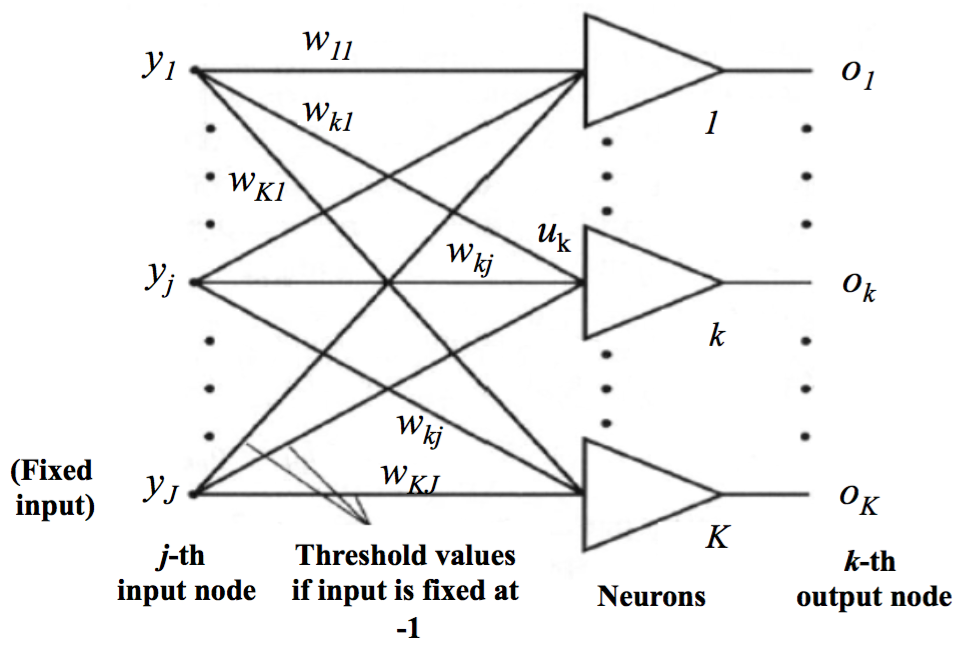
\includegraphics[width=10cm]{chapter3_mlp}
\end{figure}
\noindent Total synaptic input to the output layer:
$$\mathbf{u = Wy}$$
Output of the network:
$$\mathbf{o} = f(\mathbf{u})$$
Desired output for pattern $p$:
$$\mathbf{d_p}=(d_{p1}, d_{p2} \ldots d_{pK})^{T}$$
The error at output layer:
$$E_p=\frac{1}{2}\sum_{k=1}^{K}(d_{pk}-o_{pk})^2$$
For gradient descent update algorithm:
\begin{equation}
\triangle w_{kj} = - \alpha \frac{\partial E}{\partial w_{kj}}
\label{weight_change}
\end{equation}
By using chain rule, the gradient of error function:
\begin{equation}
\frac{\partial E}{\partial w_{kj}} = \frac{\partial E}{\partial u_k} \frac{\partial u_k}{\partial w_{kj}}
\label{error_derive_chain_rule}
\end{equation}
The \emph{error signal term} produce by the $k$ th neuron is defined as:
\begin{equation}
\delta_{ok} \equiv - \frac{\partial E}{\partial u_k}
\label{signal_term}
\end{equation}
Since
\begin{equation}
\begin{split}
u_k &= \sum_{j=1}^{J} w_{kj} y_j\\
\frac{\partial u_k}{\partial w_{kj}} &= y_j
\end{split}
\label{input_derive_mlp}
\end{equation}
Substituting \ref{signal_term} and \ref{input_derive_mlp} to \ref{error_derive_chain_rule}:
\begin{equation}
\frac{\partial E}{\partial w_{kj}} = - \delta_{ok} y_j
\label{error_derive_2}
\end{equation}
The weight adjustment in \ref{weight_change} can be rewritten:
\begin{equation}
\triangle w_{kj} = \alpha \delta_{ok} y_j
\label{weight_change_2}
\end{equation}
The error signal term can be written as:
\begin{equation}
\delta_{ok}=-\frac{\partial E}{\partial o_k}\frac{\partial o_k}{\partial u_k}
\label{signal_term_chain_rule}
\end{equation}
Since
\begin{equation}
\begin{split}
E = \frac{1}{2} \sum_{k=1}^{K} (d_k - o_k)^{2} \\
\frac{\partial E}{\partial o_k} = - (d_k - o_k)
\end{split}
\label{error_derive_mlp}
\end{equation}
And since
\begin{equation}
\begin{split}
o_k &= f(u_k) \\
\frac{\partial o_k}{\partial u_k} &= f_{k}'(u_k)
\end{split}
\label{output_derive_mlp}
\end{equation}
Subtituting \ref{output_derive_mlp} and \ref{error_derive_mlp} to \ref{error_derive_mlp}:
\begin{equation}
\begin{split}
\delta_{ok} = (d_k -o_k)f_{k}'(u_k)
\end{split}
\label{signal_term_2}
\end{equation}
Final equation of weight adjustment:
$$\triangle w_{kj} = \alpha (d_k - o_k)f_{k}'(u_k) y_j$$
The learning equation:
\begin{equation*}
\begin{split}
w_{kj}^{new} &= w_{kj}^{old} + \triangle w_{kj} \\
w_{kj}^{new} &= w_{kj}^{old} + \alpha \delta_{ok} y_j
\end{split}
\end{equation*}
Rewritten the learning equation in matrix form:
$$\mathbf{W^{new} = W^{old} + \alpha \delta_o y^{T}}$$
$$\mathbf{\delta_o = (d-o) .* f'(u)}$$

\section{Generalized Delta Learning Rule}
\begin{figure}[h]
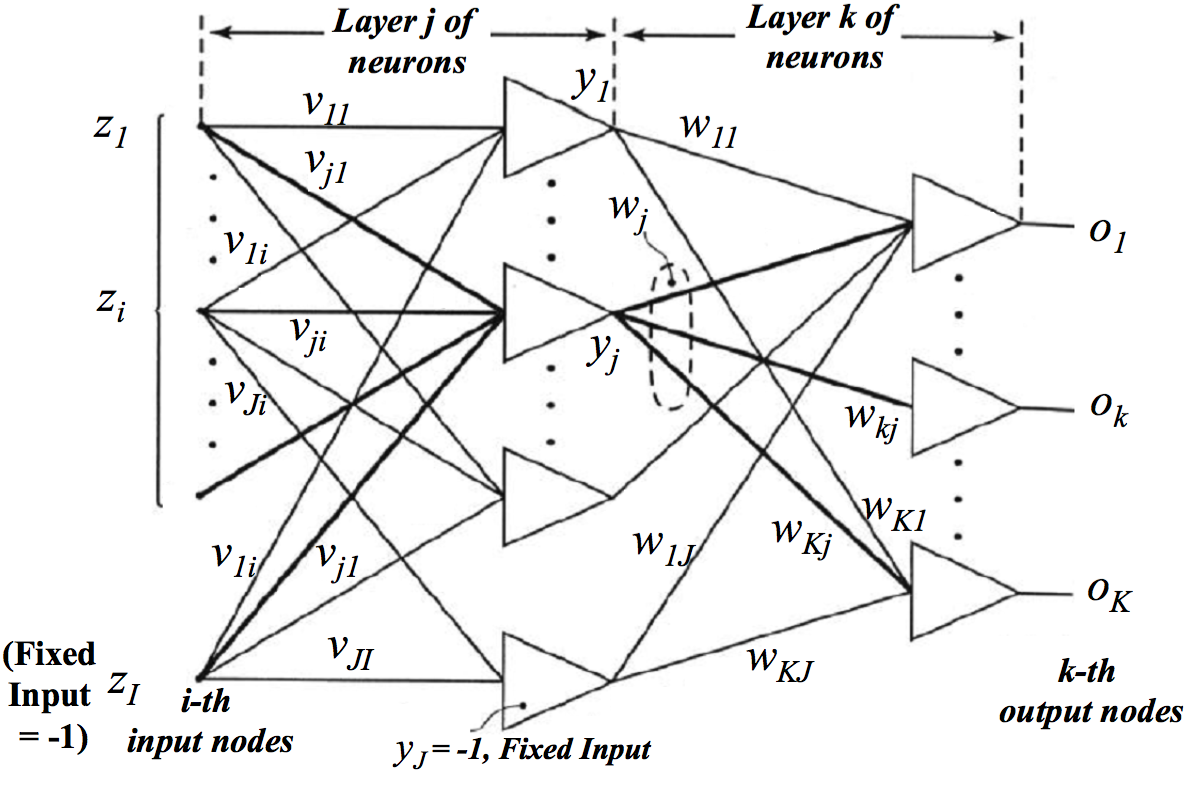
\includegraphics[width=10cm]{chapter3_mlp_2}
\end{figure}
\noindent The weight adjustment of hidden layer neurons:
\begin{equation}
\triangle v_{ji} = -\beta \frac{\partial E}{\partial v_{ji}}
\label{weight_adjust_hidden}
\end{equation}
Using chain rule:
\begin{equation}
\frac{\partial E}{\partial v_{ji}} = \frac{\partial E}{\partial s_j} \frac{\partial s_j}{\partial v_{ji}}
\label{error_derive_hidden}
\end{equation}
Since the net synaptic input to hidden layer neuron is:
\begin{equation}
\begin{split}
s_j &= \sum_{i} v_{ji} z_i\\
\frac{\partial s_j}{\partial v_{ji} } &= z_i
\end{split}
\label{input_derive_hidden}
\end{equation}
The error signal term at hidden layer is defined as:
\begin{equation}
\delta_{yj} \equiv - \frac{\partial E}{\partial s_j}
\label{error_term_hidden}
\end{equation}
Substituting \ref{input_derive_hidden} and \ref{error_term_hidden} into \ref{error_derive_hidden}:
$$\frac{\partial E}{\partial v_{ji}} = - \delta_{yj} z_i$$
Equation \ref{weight_adjust_hidden} can be written as:
$$ \triangle v_{ji} = \beta \delta_{yj} z_i $$
The error signal term in equation \ref{error_term_hidden} can be computed as:
\begin{equation}
\delta_{yj} = - \frac{\partial E}{\partial y_j} \frac{\partial y_j}{\partial s_j}
\label{error_term_derive_hidden}
\end{equation}
Where:
\begin{equation}
\begin{split}
E &= \frac{1}{2} \sum_{k=1}^{K} (d_k - f_k (u_k))^{2} \\
\frac{\partial E}{\partial y_j} &= - \sum_{k=1}^{K} (d_k - o_k) \frac{\partial}{\partial y_j} (f_k (u_k)) \\
&= - \sum_{k=1}^{K} (d_k - o_k) f_k' (u_k) \frac{\partial u_k}{\partial y_j} \\
&= - \sum_{k=1}^{K} \delta_{ok} \frac{\partial u_k}{\partial y_j}
\end{split}
\label{temp1}
\end{equation}
Since:
\begin{equation}
\begin{split}
u_k &= \sum_{j=1}^{J} w_{kj} y_j \\
\frac{\partial u_k}{\partial y_j} &= w_{kj}
\end{split}
\label{temp2}
\end{equation}
And since:
\begin{equation}
\begin{split}
y &= f(s) \\
\frac{\partial y}{\partial s_j} &= f_{j}'(s_j)
\end{split}
\label{temp3}
\end{equation}
Substituting \ref{temp1} \ref{temp2} \ref{temp3} into \ref{error_term_derive_hidden}:
$$\delta_{yj} = f_j'(s_j)\sum_{k=1}^{K} \delta_{ok} w_{kj}$$
Final equation of weight adjustment:
$$\triangle v_{ji} = \beta \delta_{yj} z_i$$
The learning equations:
\begin{equation*}
\begin{split}
v_{ji}^{new} &= v_{ji}^{old} + \triangle v_{ji} \\
v_{ji}^{new} &= v_{ji}^{old} + \beta \delta_{yj} z_i
\end{split}
\end{equation*}
Rewritten the learning equation in matrix form:
$$\mathbf{V^{new} = V^{old}} + \beta \mathbf{\delta_y z^{T}}$$
$$\mathbf{\delta_y = f'(s) .* W^{T} \delta_o}$$

\section{Application to Function Approximation}
Kolmogorov Theorem: Given any function $\mathbf{\varphi: I^{n} \rightarrow R^{m}, \varphi(x) = y}$ where $I$ is the closed unit interval [0, 1], $\phi$ can be implemented exactly by a three layer neural network with $n$ input node, $2n+1$ hidden layer neurons and $m$ output layer neurons
